\documentclass[../2.tex]{subfiles}
\begin{document}

We now proceed by analogy with the previous section and define a \ii{discrete Dirichlet energy} on graphs, using the laplacian matrix written on the canonical basis, as
in definition \ref{lapdef}.
Our reference for this part is \cite{bronstein}.

\begin{defn}
    Let $A,\Phi$ be to $n\times n$ matrices, we define the \ii{discrete Dirichlet energy} to be 
    \[ D[\Phi] = \tr(\Phi^T \Delta_0 \Phi). \]
\end{defn}

Notice the analogy with the setting as expressed by proposition \ref{prop:2:4:3}.
In the following treatment we will simply use $\Delta$ for the $0$-laplacian.

We have already seen that the $0$-laplacian can be represented as a matrix with respect to the canonical basis
of $0$-chains. Let us now see a more efficient way to compute the $0$-laplacian matrix. In order to do that we need to introduce some notation.

\begin{defn}
    Let $\mc{G}$ be a simple undirected graph, let $\ch{i} \in C_0$ we define the \ii{degree} of $\ch{i}$ to be 
    \[ \dg(i) := \sum_{j : \ch{i,j} \in C_1} 1. \]
\end{defn}

According to this definition the degree of a vertex of a graph is the number of vertices that vertex is linked to by an edge.

\begin{prop}
    The laplacian matrix on the canonical basis of $0$-chains can be written as
    \[ \Delta = D - A, \]
    where $D_{ij} := \delta_{ij}deg(i)$ is the degree matrix and $A$ is the adjacency matrix.
    \label{prop:d-a}
\end{prop}
\begin{proof}
    This proposition is an immediate consequence of definition \ref{def:2:2:2}. \qedhere
\end{proof}

The connstruction of this same matrix in the example \ref{ex:2:3:2} was presented to become aquainted with the abstract definition of laplacian operators.
Proposition \ref{prop:d-a} actually gives the most efficient way to write the $0$-laplacian matrix for any simple undirected graph.

It is easy to see that graphs with multiple connected componets the $0$-laplacian matrix is a block matrix whose blocks are the laplacians of the connected components.

Let's now focus on a connected graph or in alternative on a single connected component of an unconnected graph. What are the properties of this matrix?
The $i$-th coloumn of the matrix has $\dg{i}$ on the $i$-th row and $-1$ on the $j$-th row if $\ch{i,j} \in C_1$. If we recall the definition of degree of a vertex
it is immediate to understand that the sum of the elements of a coloumn is always zero, therefore the sum of the rows is also zero. From these considerations
we derive the following proposition.\\
\hfill \\

The minimization of the discrete Dirichlet energy is not a variational problem, rather a simple minimization in $\Phi$ in which we can 
use the standard Lagrange multipliers theorem. Here the $0$-laplacian is a matrix instead of a differential operator. 
\begin{prop}
    The minimum for the Dirichlet energy $ \tr(\Phi^T \Delta \Phi)$ constrained to the $\Phi$ such that $\Phi^T \Phi = 1$ is reached when the
    rows of $\Phi$ are the laplacian eigenvectors.
\end{prop}
\begin{proof}
    The Lagrange multipliers' theorem allows us to use costraints by minimizing the following constrained Dirichlet energy
    \[ D[\Phi] = \sum_{i,j,k} \Phi_{ik} \Delta_{ij} \Phi_{jk} - \sum_{i,j,k} \Lambda_{ij} \Phi_{kj} \Phi_{ki}, \]
    where $\Lambda$ is a diagonal matrix with the Lagrange multipliers as eigenvalues.\\
    In fact the constraints $\Phi^T \Phi = 1$ can be written as $\sum_k \Phi_{kj} \Phi{ki} = \delta_{ij}$, therefore I need to subtract from my lagrangian
    the quantity $\sum_{i,j} \sum_k \Lambda_{ij} \Phi_{kj} \Phi{ki}$. Actually because of the constraint itself I already now that for $i \neq j$ the quantity
    I am substracting from the lagrangian vanishes, therefore we can see $\Lambda$ as a diagonal matrix of lagrange multipliers.  

    We then minimize this energy
    \[ \frac{\del D[\Phi]}{\del \Phi_{mn}} = \sum_{i,j,k} \delta_{im}\delta_{nk}\Delta_{ij} \Phi_{jk} + \sum_{i,j,k} \Phi_{ik} \Delta_{ij}\delta_{jm}\delta_{nk}
    - \sum_{i,j,k} \Lambda_{ij} \delta_{mk}\delta_{nj}\Phi_{ki} - \sum_{i,j,k} \Lambda_{ij} \Phi_{kj} \delta_{mk}\delta_{ni} =  \]
    \[ = \sum_{j} \Delta_{mj} \Phi_{jn} + \sum_{i} \Phi_{in} \Delta_{im} - \sum_{i} \Lambda_{in} \Phi_{mi} - \sum_{j} \Lambda_{nj} \Phi_{mj} = 0, \]
    which using the symmetry of $\Lambda$ and $A$ can be written as
    \[ \sum_{j} \Delta_{mj} \Phi_{jn} + \sum_{i}  \Delta_{mi} \Phi_{in} - \sum_{i} \Phi_{mi}\Lambda_{in} - \sum_{j} \Phi_{mj} \Lambda_{jn} =  \]
    \[ 2\Delta\Phi - 2\Phi\Lambda = 0. \]
    We then obtain 
    \[ \Delta\Phi = \Phi\Lambda, \]
    which for every row of $\Phi$ is an eigenvalue equation. \qedhere
\end{proof}

\begin{figure}[H]
    \centering
    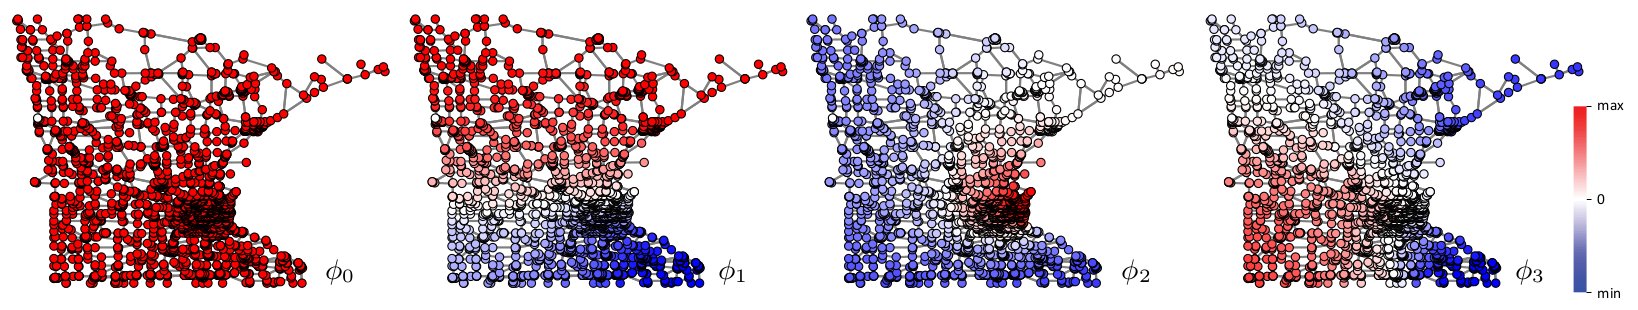
\includegraphics[width=17cm, height=4cm]{sections/2/eiglap}
    \caption{A graphical representation of the first laplacian eigenchains on the Minnesota Road Graph.
    The color of a node $\ch{i}$ represents the value $\braket{i}{\phi_j}$ of the $0$-laplacian eigenfunction $\ch{\phi_j}$
    on the node.}
    \label{fig:2:5}
\end{figure}

In figure \ref{fig:2:5} we can see some of the $0$-laplacian eigenfunctions. We notice that the eigenfunction corresponding to the eigenvalue $0$ is uniform.

\begin{prop}
    Let $\mc{G}$ be a simple undirected connected graph then 
    \[ \sum_{C_0} \ch{i} \in \ker\Delta. \]
\end{prop}

Since according to Eckmann's theorem the dimension of the kernel of the $0$-laplacian for a simple connected graph should be one, 
we have that $\sum_{C_0} \ch{i}$ is the only linearly independent chain in the kernel, therefore the unique $0$-laplacian eigenfunction
with eigenvalue zero up to scalar multiplication. Since the coefficients in the formal sum of the basis $0$-chains are all equal, we have that the $0$-laplacian eigenchain
of a simple undrected connected graph is always uniform as in fig. \ref{fig:2:5}.

    
\end{document}